\section[Materials]{Materials}
\label{sec:materials}

\subsection[XGBoost classifier to uncover the function of lncRNAs in cell-growth]{XGBoost classifier to uncover the function of lncRNAs in cell-growth}
\label{sec:genome_datasets}

CRISPRi library was obtained from Liu \textit{et al.}\autocite{liu_2017_crispri} work (\autoref{tab:crispri-lib}). Additionally, 124 transcription factors (TFs) were downloaded from ENCODE\autocite{encode_2004,encode_2011_user} to train and test different machine learning (ML) models (\autoref{tab:encode-tfs}).

\begin{table}[!htb]
  \caption[CRISPRi library]{\textbf{CRISPRi library}}
  \begin{scriptsize}
    \begin{tabulary}{0.95\linewidth}{cccccccc}
      \multicolumn{1}{c}{\textbf{Cell line}} & \textbf{Number of hits} & \textbf{Targeted loci} & \multicolumn{1}{|c}{\textbf{Cell line}} & \textbf{Number of hits} & \textbf{Targeted loci} \\ \hline
      HEK293T & \multicolumn{1}{r}{28} & \multicolumn{1}{r}{5,615}  & \multicolumn{1}{|c}{MCF7} & \multicolumn{1}{r}{117} & \multicolumn{1}{r}{5,725}  \\
      HeLa & \multicolumn{1}{r}{52} & \multicolumn{1}{r}{6,158}  & \multicolumn{1}{|c}{MDAMB231} & \multicolumn{1}{r}{44} & \multicolumn{1}{r}{5,725}  \\
      iPSC  & \multicolumn{1}{r}{438} & \multicolumn{1}{r}{5,534}  & \multicolumn{1}{|c}{U87} & \multicolumn{1}{r}{88} & \multicolumn{1}{r}{5,689}  \\
      K562 & \multicolumn{1}{r}{144} & \multicolumn{1}{r}{16,401}  & \multicolumn{1}{|c}{} & \multicolumn{1}{r}{} & \multicolumn{1}{r}{}  \\
    \end{tabulary}
  \end{scriptsize}
  \label{tab:crispri-lib}
\end{table}

\begin{table}[!htb]
  % \caption[]{}
  \begin{scriptsize}
    \begin{tabulary}{0.95\linewidth}{ccccccc}
      \textit{ARID3A} & \textit{ATF1} & \textit{ATF2} & \textit{ATF3} & \textit{BACH1} & \textit{BCLAF1} & \textit{BHLHE40} \\
      \textit{BRCA1} & \textit{CBX3} & \textit{CBX8} & \textit{CEBPB} & \textit{CEBPZ} & \textit{CHD1} & \textit{CHD2}   \\
      \textit{CHD7}  &  \textit{CREB1} & \textit{CTBP2} & \textit{CTCF} &  \textit{CTCFL} &  \textit{CUX1} &   \textit{E2F1}   \\
      \textit{E2F4}  &  \textit{E2F6} &   \textit{EGR1}  &  \textit{ELF1} & \textit{ELK1} &  \textit{EP300} & \textit{ESRRA}  \\
      \textit{ETS1} &   \textit{EZH2}  &  \textit{FOS}  &  \textit{FOSL1} &  \textit{FOSL2} &  \textit{FOXA1} &  \textit{FOXM1}  \\
      \textit{GABPA} &  \textit{GATA1} &  \textit{GATA2} &  \textit{GATA3} &  \textit{GTF2F1} &  \textit{HCFC1} &  \textit{HDAC1}  \\
      \textit{HDAC2}  &  \textit{HDAC6} &  \textit{HSF1} &   \textit{IKZF1} &  \textit{IRF1}  &  \textit{JUN}  &   \textit{JUND}   \\
      \textit{KDM1A} & \textit{KDM5A} &  \textit{KDM5B} &  \textit{MAFF} & \textit{MAFK} & \textit{MAX} & \textit{MAZ} \\
      \textit{MEF2A} &  \textit{MTA3} &  \textit{MXI1} &   \textit{MYBL2} &  \textit{MYC} &  \textit{NANOG} & \textit{NCOR1}  \\
      \textit{NFE2} &  \textit{NFIC} &  \textit{NFYA} &  \textit{NFYB} &  \textit{NR2C2} & \textit{NR2F2} &  \textit{NR3C1}  \\
    \end{tabulary}
  \end{scriptsize}
  \label{tab:encode-tfs-first-part}
\end{table}

\begin{table}[!htb]
  \caption[ENCODE TFs]{\textbf{ENCODE TFs}. 124 TFs from the ENCODE project.\autocite{encode_2004,encode_2011_user}}
  \begin{scriptsize}
    \begin{tabulary}{0.95\linewidth}{ccccccc}
      \textit{NRF1} &   \textit{PHF8} &  \textit{PML}  &  \textit{POLR2A} & \textit{POU5F1} &  \textit{RAD21}  &  \textit{RBBP5}  \\
      \textit{RCOR1} &  \textit{RELA} &  \textit{REST} &  \textit{RFX5} &  \textit{RNF2}  &  \textit{RXRA}  & \textit{SAP30}  \\
      \textit{SETDB1} &  \textit{SIN3A} &  \textit{SIX5} &  \textit{SMARCA4} & \textit{SMARCB1} & \textit{SMARCC2} & \textit{SMC3}   \\
      \textit{SP1} & \textit{SPI1}  & \textit{SREBF1} & \textit{SREBF2} & \textit{SRF} & \textit{STAT5A} & \textit{SUPT20H} \\
      \textit{SUZ12} & \textit{TAF1}  &  \textit{TAF7} &  \textit{TAL1} & \textit{TBL1XR1} & \textit{TBP}  &  \textit{TCF12}  \\
      \textit{TCF7L2} &  \textit{TEAD4} &  \textit{THAP1} &  \textit{TRIM28}  & \textit{UBTF} & \textit{USF1} & \textit{USF2}   \\
      \textit{YY1} & \textit{ZBTB33} & \textit{ZBTB7A} & \textit{ZC3H11A} & \textit{ZKSCAN1} & \textit{ZMIZ1} & \textit{ZNF143} \\
      \textit{ZNF217} & \textit{ZNF263} & \textit{ZNF274} & \textit{ZNF384} & \textit{ZZZ3} \\
    \end{tabulary}
  \end{scriptsize}
  \label{tab:encode-tfs}
\end{table}

\subsection{LncRNA analysis of the \textit{Drosophila} genome during regeneration}
\label{sec:genome_datasets_first_part}

\subsubsection{Characterization of cell-damage lncRNAs}
\label{sec:materials-dme-one}

Regeneration data was acquired from Vizcaya-Molina \textit{et al.} study\autocite{vizcaya_2018} under GEO accession number: GSE102841. \autoref{tab:regeneration-dataset} indicates type of genome-wide technique, organism, tissue, and condition. In this thesis work, terms 0h and early, 15h and mid, and 25h and late terms were used interchangeably. 

\begin{table}[!htb]
  \caption[Regeneration data]{\textbf{Regeneration data}}
  \begin{scriptsize}
    \begin{tabulary}{0.95\linewidth}{cccccc}
      \textbf{Technique} & \textbf{Organism} & \textbf{Tissue} & \textbf{Condition} & \textbf{Reference} \\ \hline
      RNA-seq & \textit{D. melanogaster} & Wing disc, 0h, 15h and 25h & Injured and Uninjured & \autocite{vizcaya_2018} \\
      H3K4me1 ChIP-seq & \textit{D. melanogaster} & Wing disc, 0h & Injured and Uninjured & \autocite{vizcaya_2018}   \\
      H3K27ac ChIP-seq & \textit{D. melanogaster} & Wing disc, 0h & Injured and Uninjured & \autocite{vizcaya_2018}   \\
      RNA Pol-II ChIP-seq & \textit{D. melanogaster} & Wing disc, 0h & Injured and Uninjured & \autocite{vizcaya_2018}   \\
      ATAC-seq & \textit{D. melanogaster} & Wing disc, 0h, 15h and 25h & Injured and Uninjured & \autocite{vizcaya_2018}  \\
    \end{tabulary}
  \end{scriptsize}
  \label{tab:regeneration-dataset}
\end{table}

\subsubsection{LncRNA developmental and tissue signatures}
\label{sec:materials-dme-two}

Developmental gene expression of \textit{Drosophila melanogaster} (\textit{D. melanogaster}) across embryonic, larval, white pre-pupal (WPP), and pupal stages were obtained from the modENCODE project\autocite{celniker_2009,modencode_2010} (\autoref{tab:developmental}).
  
\begin{table}[!htb]
  \caption[\textit{D. melanogaster} developmental data]{\textbf{\textit{D. melanogaster} developmental data}}
  \begin{scriptsize}
    \begin{tabulary}{0.95\linewidth}{ccCcCc}
      \textbf{Condition} & \textbf{Time point} & \textbf{Organism} & \textbf{Technique} & \textbf{Reference} \\ \hline
      Development & Embryo, 0h-24h  &  \textit{D. melanogaster} & RNA-seq & \autocite{celniker_2009,modencode_2010}   \\
      Development & L1, L2 and L3 & \textit{D. melanogaster} & RNA-seq & \autocite{celniker_2009,modencode_2010}  \\
      Development & WPP  & \textit{D. melanogaster}  & RNA-seq & \autocite{celniker_2009,modencode_2010} \\
      Development & Pupae, 12h-4days & \textit{D. melanogaster} & RNA-seq & \autocite{celniker_2009,modencode_2010}  \\
    \end{tabulary}
  \end{scriptsize}
  \label{tab:developmental}
\end{table}

In addition, leg and wing imaginal discs data was obtained from Pérez-Lluch \textit{et al.}\autocite{perez_blister} work. Antenna and eye imaginal disc reads were obtained from the Roderic Guigó's lab at the Centre de Regulació Genòmica (CRG, Barcelona, Spain). Antenna, eyen, leg and wing imaginal disc data was produced in three \textit{D. melanogaster} developmental time points L3, WPP and late pupae (4.5 days pupae, see \autoref{tab:erc-rna-seq}}).

\begin{table}[!htb]
  \caption[\textit{D. melanogaster} imaginal disc data]{\textbf{\textit{D. melanogaster} imaginal disc data}}
  \begin{scriptsize}
    \begin{tabulary}{0.95\linewidth}{ccCcCc}
      \textbf{Imaginal disc} & \textbf{Time point} & \textbf{Organism} & \textbf{Technique} & \textbf{Reference}\\ \hline
      Antenna & L3, WPP and LP & \textit{D. melanogaster} & RNA-seq & NA \\
      Eye & L3, WPP and LP & \textit{D. melanogaster} & RNA-seq & NA \\
      Leg & L3, WPP and LP & \textit{D. melanogaster} & RNA-seq & \autocite{perez_blister} \\
      Wing & L3, WPP and LP & \textit{D. melanogaster} & RNA-seq & \autocite{perez_blister} \\
    \end{tabulary}
  \end{scriptsize}
  \label{tab:erc-rna-seq}
\end{table}

\subsubsection{Assessing the lncRNA:\textit{CR40469} function during \textit{D. melanogaster} imaginal-disc regeneration-process}
\label{sec:materials-dme-three}

The lncRNA \textit{CR40469} knockout (KO) data contains the lncRNA \textit{CR40469} knocked-out (\textit{CR40469}$^{KO}$) and the lncRNA \textit{CR40469} in wild-type (\textit{CR40469}$^{Wt}$) within control and regeneration conditions both at the early time point (0h, \autoref{tab:cr40469-ko}). 

\begin{table}[!htb]
  \caption[\textit{CR40469} knockout data]{\textbf{\textit{CR40469} knockout data}}
  \begin{scriptsize}
    \begin{tabulary}{0.95\linewidth}{ccCcCc}
      \textbf{Genotype} & \textbf{Condition} & \textbf{Tissue} & \textbf{Organism} & \textbf{Technique} & \textbf{Reference} \\ \hline
      \textit{CR40469}$^{Wt}$ & Uninjured & Wing disc, 0h & \textit{D. melanogaster} & RNA-seq & NA \\
      \textit{CR40469}$^{KO}$  &  Uninjured & Wing disc, 0h & \textit{D. melanogaster} & RNA-seq & NA \\
      \textit{CR40469}$^{Wt}$  &  Injured & Wing disc, 0h & \textit{D. melanogaster} & RNA-seq & NA \\
      \textit{CR40469}$^{KO}$  &  Injured & Wing disc, 0h & \textit{D. melanogaster} & RNA-seq & NA \\
    \end{tabulary}
  \end{scriptsize}
  \label{tab:cr40469-ko}
\end{table}

\clearpage

\section[Methods]{Methods}

\subsection[XGBoost classifier to uncover the function of lncRNAs in cell-growth]{XGBoost classifier to uncover the function of lncRNAs in cell-growth}
\label{sec:ml_methods}

\subsubsection{Data gathering and preprocessing}
\label{sec:ml_data}

\paragraph{CRISPRi data}
\label{sec:crispr_i_methods}

CRISPRi data was obtained from Liu \textit{et al.}\autocite{liu_2017_crispri} targeting 16,401 lncRNA transcripts from seven human cell lines: iPSC, K562, U87, MCF7, MDA-MB-231, HeLa, and HEK293T; and 18 genomic features: expression level in log$_2$(FPKM + 0.1), near FANTOM enhancer, near cancer associated SNP, number of exons, within \textit{Pol2} loop, near super enhancer, within \textit{CTCF} loop, near traditional enhancer, has mouse ortholog, locus is heterozygous deleted, is intergenic, transcript length, locus is amplified, is antisense, locus-nearest coding gene distance, TSS-nearest coding distance, near VISTA enhancer, and locus is homozygous deleted.

LncRNA hit is defined if inhibiting its transcriptional expression modifies cell-growth, either positively or negatively.\autocite{liu_2017_crispri} See \autoref{fig:ml-workflow} to have a general overview. 

\paragraph{ENCODE TF ChIP-seq}
\label{sec:encode_methods}

We used ENCODE TF ChIP-seq data\autocite{encode_2004,encode_2011_user} to determine transcription factor peak height within lncRNA promoters across five cell lines: HEK293T, HeLa, MCF7, K562 and H1-hESC, using 124 transcription factors (TFs).

We downloaded the bigBed narrowPeak files with optimal irreproducible discovery rate (IDR) thresholded peaks in hg19 assembly coordinates. We applied a window of [-300; +100] bp upstream and downstream, respectively at the TSS to obtain lncRNA promoters, according to Dao \textit{et al.}\autocite{dao_2017} Then using \textit{BEDTools} \autocite{quinlan_2010_bedtools} intersect v2.27, TFs bigBed, and lncRNA promoters bed file the TF peak height was obtained. A 10\% intersection cutoff between TF ChIP-seq and lncRNA promoter was used. 

\subsubsection{Model training}
\label{sec:ml_part}

Stratified 10-fold cross-validation with 3 different randomizations in each repetition was adopted to train all supervised models, using the \textit{RepeatedStratifiedKFold} class from \textit{scikit-learn}\autocite{pedregosa_2011_scikit} version 0.24.1, with 90\% and 10\% for training and test, respectively (see \autoref{fig:ml-process}). Ensuring the training and the test sets to have the same hit proportion as the original dataset.

\begin{figure}[!htb]
  \centering
  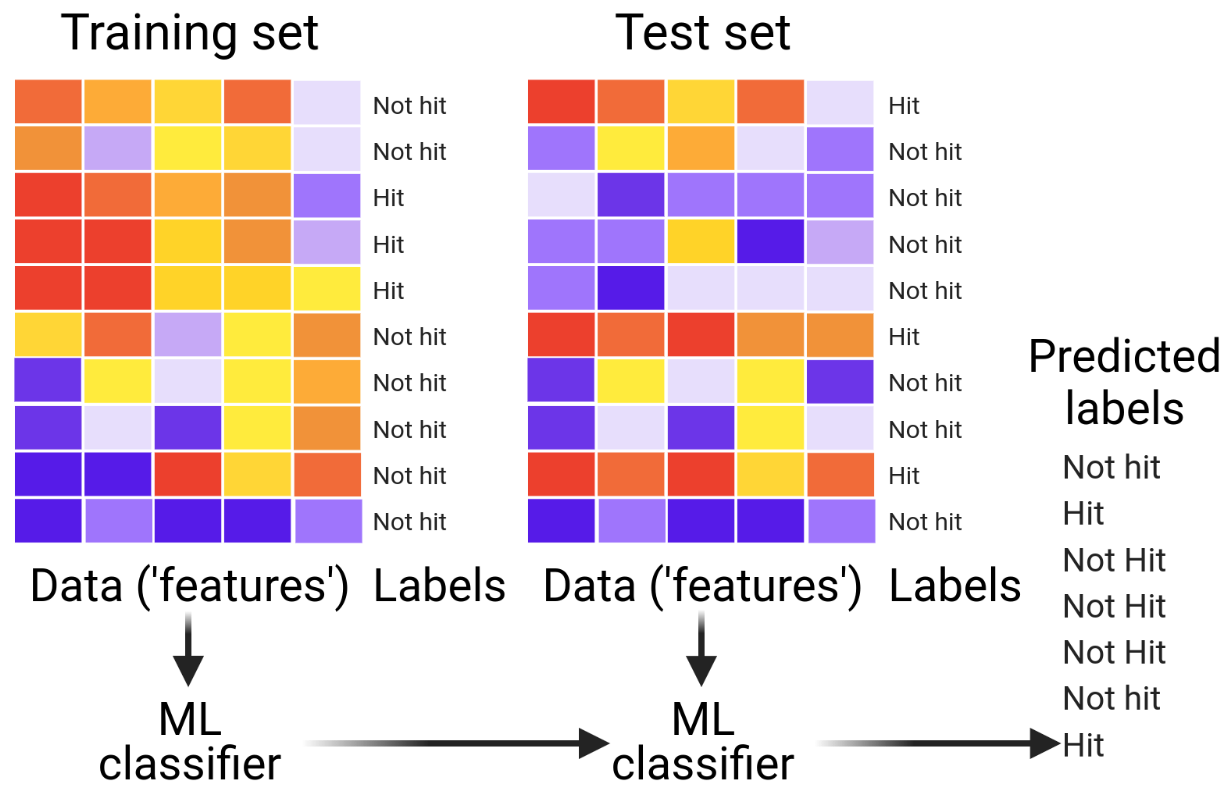
\includegraphics[width=0.6\textwidth]{img/methods/ml_project/ml_process.png}
  \caption[Process followed for model training]{\textbf{Process followed for model training}. The functional screening based on CRISPRi and the ENCODE Transcription Factor datasets were splitted into 90\% for the training set (adopting a stratified cross-validation) and 10\% for the testing set; along with binary labels indicating whether the lncRNA locus is either a hit or not hit.}
  \label{fig:ml-process}
\end{figure}

\paragraph{XGBoost}
\label{sec:XGBoost_methods}

The \textit{dmlc XGBoost} library (\url{https://xgboost.readthedocs.io/en/latest/index.html}) version 1.3.3 was used for implementing the XGBoost\autocite{chen_2016_xgboost} model. XGBoost is a type of gradient boosting decision tree method; its objective function is defined as follows:

\[ L(\phi)= \sum_{n=1}^n loss(y_i, \hat{y_i}) + \sum_{k=1}^K \Omega(f_k)  \]

where loss is the logistic regression for binary classification (\textit{binary:logistic}), $\Omega(f_k) $is the complexity of the tree, and K is the number of trees in the model. The machine learning method, XGBoost, was tuned to search for an optimal sensitivity and specificity solution. To tune the hyper-parameters, we adopted the \textit{GridSearchCV} \textit{scikit-learn}\autocite{pedregosa_2011_scikit} class to improve the performance of the model, using a NVIDIA GPU \textit{GeForce RTX-2060} (drivers version= 465.31, and CUDA version= 11.3). The hyper-parameters tuned for XGBoost control the growth and the robustness of the model and were the following:

\begin{itemize}
\item Growth: learning rate, max depth, and regularization lambda.
\item Robustness: gamma.
\end{itemize}

\paragraph{Logistic regression}
\label{sec:logit_methods}

\textit{Scikit-learn}\autocite{pedregosa_2011_scikit} \textit{LogisticRegression} was implemented for the logistic regression model. \textit{C values} and penalty hyper-parameters were tuned using \textit{GridSearchCV}.

\begin{itemize}
\item \textit{C value}: inverse of regularization strength, smaller c values means stronger regularization. 
\item Penalty: Lasso $(l_1)$, and Ridge $(l_2)$ applying square and absolute transformation on the model coefficients, respectively. 
\end{itemize}

\paragraph{Balanced random forest}
\label{sec:logit_methods}

We used a random forest modification to perform data resampling on the bootstrap sample to change the class distribution. The \textit{BalancedRandomForestClassifier} class from the \textit{imbalanced-learn}\autocite{lemaitre_2017_imbalanced} python library, version 0.8.0, implements this and performs random under-sampling of the majority class (\textit{i.e.} not hits) in each bootstrap sample. The balanced random forest was implemented with default parameters. 

\paragraph{Cost-sensitive methods}
\label{sec:cost-sensitive-methods}

As our dataset was unbalanced, the ratio of the minority positive class (hits) versus the majority negative class (not hits) was 1/55, we adopted the XGBoost \textit{scale position weight} parameter to train a cost-sensitive XGBoost classifier for imbalanced data, 54.81 (default scale position weight) , 100, and 1000 values were used for grid search. 

\[ default\ scale\ postion\ weight= \frac{sum(majority\ negative\ class)}{sum(minority\ positive\ class)} \]

For the class-weight logistic regression model the inverse of the class distribution was used, by passing \textit{balanced} as the input to the logistic regression \textit{class\_weight} parameter.

The final tuning results for cost-sensitive XGBoost and cost-sensitive logistic regression were the following:

\begin{table}[!htb]
  \caption[Cost-sensitive results]{\textbf{Cost-sensitive parameters}}
  \begin{scriptsize}
    \begin{tabulary}{0.95\linewidth}{CCC}
      \multicolumn{3}{c}{\textbf{Cost-sensitive XGBoost}} \\ \hline
      Learning rate= 0.05 & Max depth= 5 & Regularization lambda= 5.0 \\
      Scale position weight= 100 & Gamma= 1.0 \\
      \multicolumn{3}{c}{\textbf{Cost-sensitive Logistic regression}} \\ \hline
      C value= 1.0 & Penalty= $l2$ & Class weight =balanced 
    \end{tabulary}
  \end{scriptsize}
  \label{tab:cost-sensitive-xgboost}
\end{table}

\paragraph{Sampling methods}
\label{sec:under-sampling-methods}

We adopted random majority under-sampling with and without replacement to re-sample our training and test sets, which reduced the impact of data imbalance.  The python package \textit{imbalanced-learn}\autocite{lemaitre_2017_imbalanced} version 0.8.0 was used to implement the random majority under-sampling method.  

The following sampling strategy values were used: 3\%, 4\%, 5\%, 10\%, 20\%, 30\%, 40\% and 50\%.

\paragraph{Metrics}
\label{sec:metrics_methods}

Further, to evaluate all model performance’s, we measured the sensitivity (recall), specificity, precision, F1 score, AUROC, Brier score, and Brier skill score, using the stratified 10-fold cross-validation process described above (see \nameref{sec:ml_part}). 

Sensitivity is the ratio of correctly predicted positive observations to all observations in a specific class, and aims to minimize the number of false negatives. It was calculated as follows in terms of the confusion matrix:

\[ Sensitivity= \frac{TP}{TP+FN}  \]

Specificity is the ratio of correctly predicted negative observations to all observations in a specific class, and it was obtained as:

\[ Specificity= \frac{TN}{TN+FP} \]

Precision is the ratio of correctly predicted positive observations to total predicted positive observations, aims to minimize the number of false positives, and was calculated using the following equation:

\[ Precision= \frac{TP}{TP+FP}  \]

F1 score is the weighted average of precision and sensitivity, maximize both precision and sensitivity, and was calculated as follows:

\[ F1\ score= 2*\frac{Sensitivity*Precision}{Sensitivity+Precision}  \]

Brier score is a mean square error criterion applied to binary data, and was measured as: 

\[ Brier\ score= \frac{1}{n}\sum_{i=1}^n(y_i-\hat{y_i})^2  \]

$\hat{y_i}$ is the predicted probabilities given to a set of $n$ binary observations, and $y_i$ taking on values 0 and 1. Brier score ranges between 0 and 1, with 0 being the score of a perfectly skilled classifier. Brier skill score is a relative metric used to compare models, a negative value means decreased performance compared to the reference. It was implemented as follows: 

\[ Brier\ skill\ score= 1 - (\frac{Brier\ score}{ref.\ Brier\ score}) \]

\subsubsection{Recursive feature elimination (RFE)}
\label{sec:rfe_methods}

Recursive feature elimination (RFE) removing the lowest importance features, based on SHAP values\autocite{lundberg_2020, lundberg_2018} with stratified cross-validation was implemented using the \textit{ShapRFECV} class from the \textit{probatus} python library (\url{https://ing-bank.github.io/probatus/index.html}), version 1.8.4.  The step was one feature per iteration, and using sensitivity and specificity as scoring metrics. 

\subsubsection{Model explainability and predictions}
\label{sec:model_explanation_methods}

\textit{TreeExplainer} from the SHapley Additive exPlanations\autocite{lundberg_2020, lundberg_2018} (SHAP) framework version 0.39.0 has been used to explain the output of our XGBoost model. Global and local explanations were obtained based on 10\% of the data not used to train our algorithm. The SHAP framework is based on Shapley values\autocite{shapley_SHAP_values}, which is a cooperative game theory concept introduced by Shapley. 

To generate a list of lncRNA candidates for experimental evaluation, we used our cost-sensitive XGBoost model with 71 features to predict hit probabilities using the whole CRISPRi library. 

\subsubsection{Experimental evaluation}
\label{sec:prediction_exp_eva_methods}

The lncRNA \textit{LINC00879} was knocked-down using CRISPRi. Two synthetic guide RNAs (sgRNAs) were retrieved from Liu \textit{et al.}\autocite{liu_2017_crispri} sgRNA table, and clone them into \textit{pCRISPRia-v2.0} plasmid which includes the blue-fluorescent-protein (BFP). 

For competitive growth assay, we mixed cells expressing mCherry and BFP containing the two sgRNAs targeting the lncRNA of interest or the non-targeting control at 50\%. Flow cytometry was used to measure the change of BFP$^+$ cells fraction over 7 days.  Three technical replicates were used and knockdown was validated using qPCR. (\textit{These experiments were carried out by Joshua Hazan, from Assaf Bester's lab at Technion-Israel Institute of Technology; Haifa, Israel}). To assess differences between cells with sgRNAs and negative controls multiple paired \textit{t-test} and \textit{Bonferroni} \textit{p-value} correction were used. 

\begin{figure}[!htb]
  \centering
  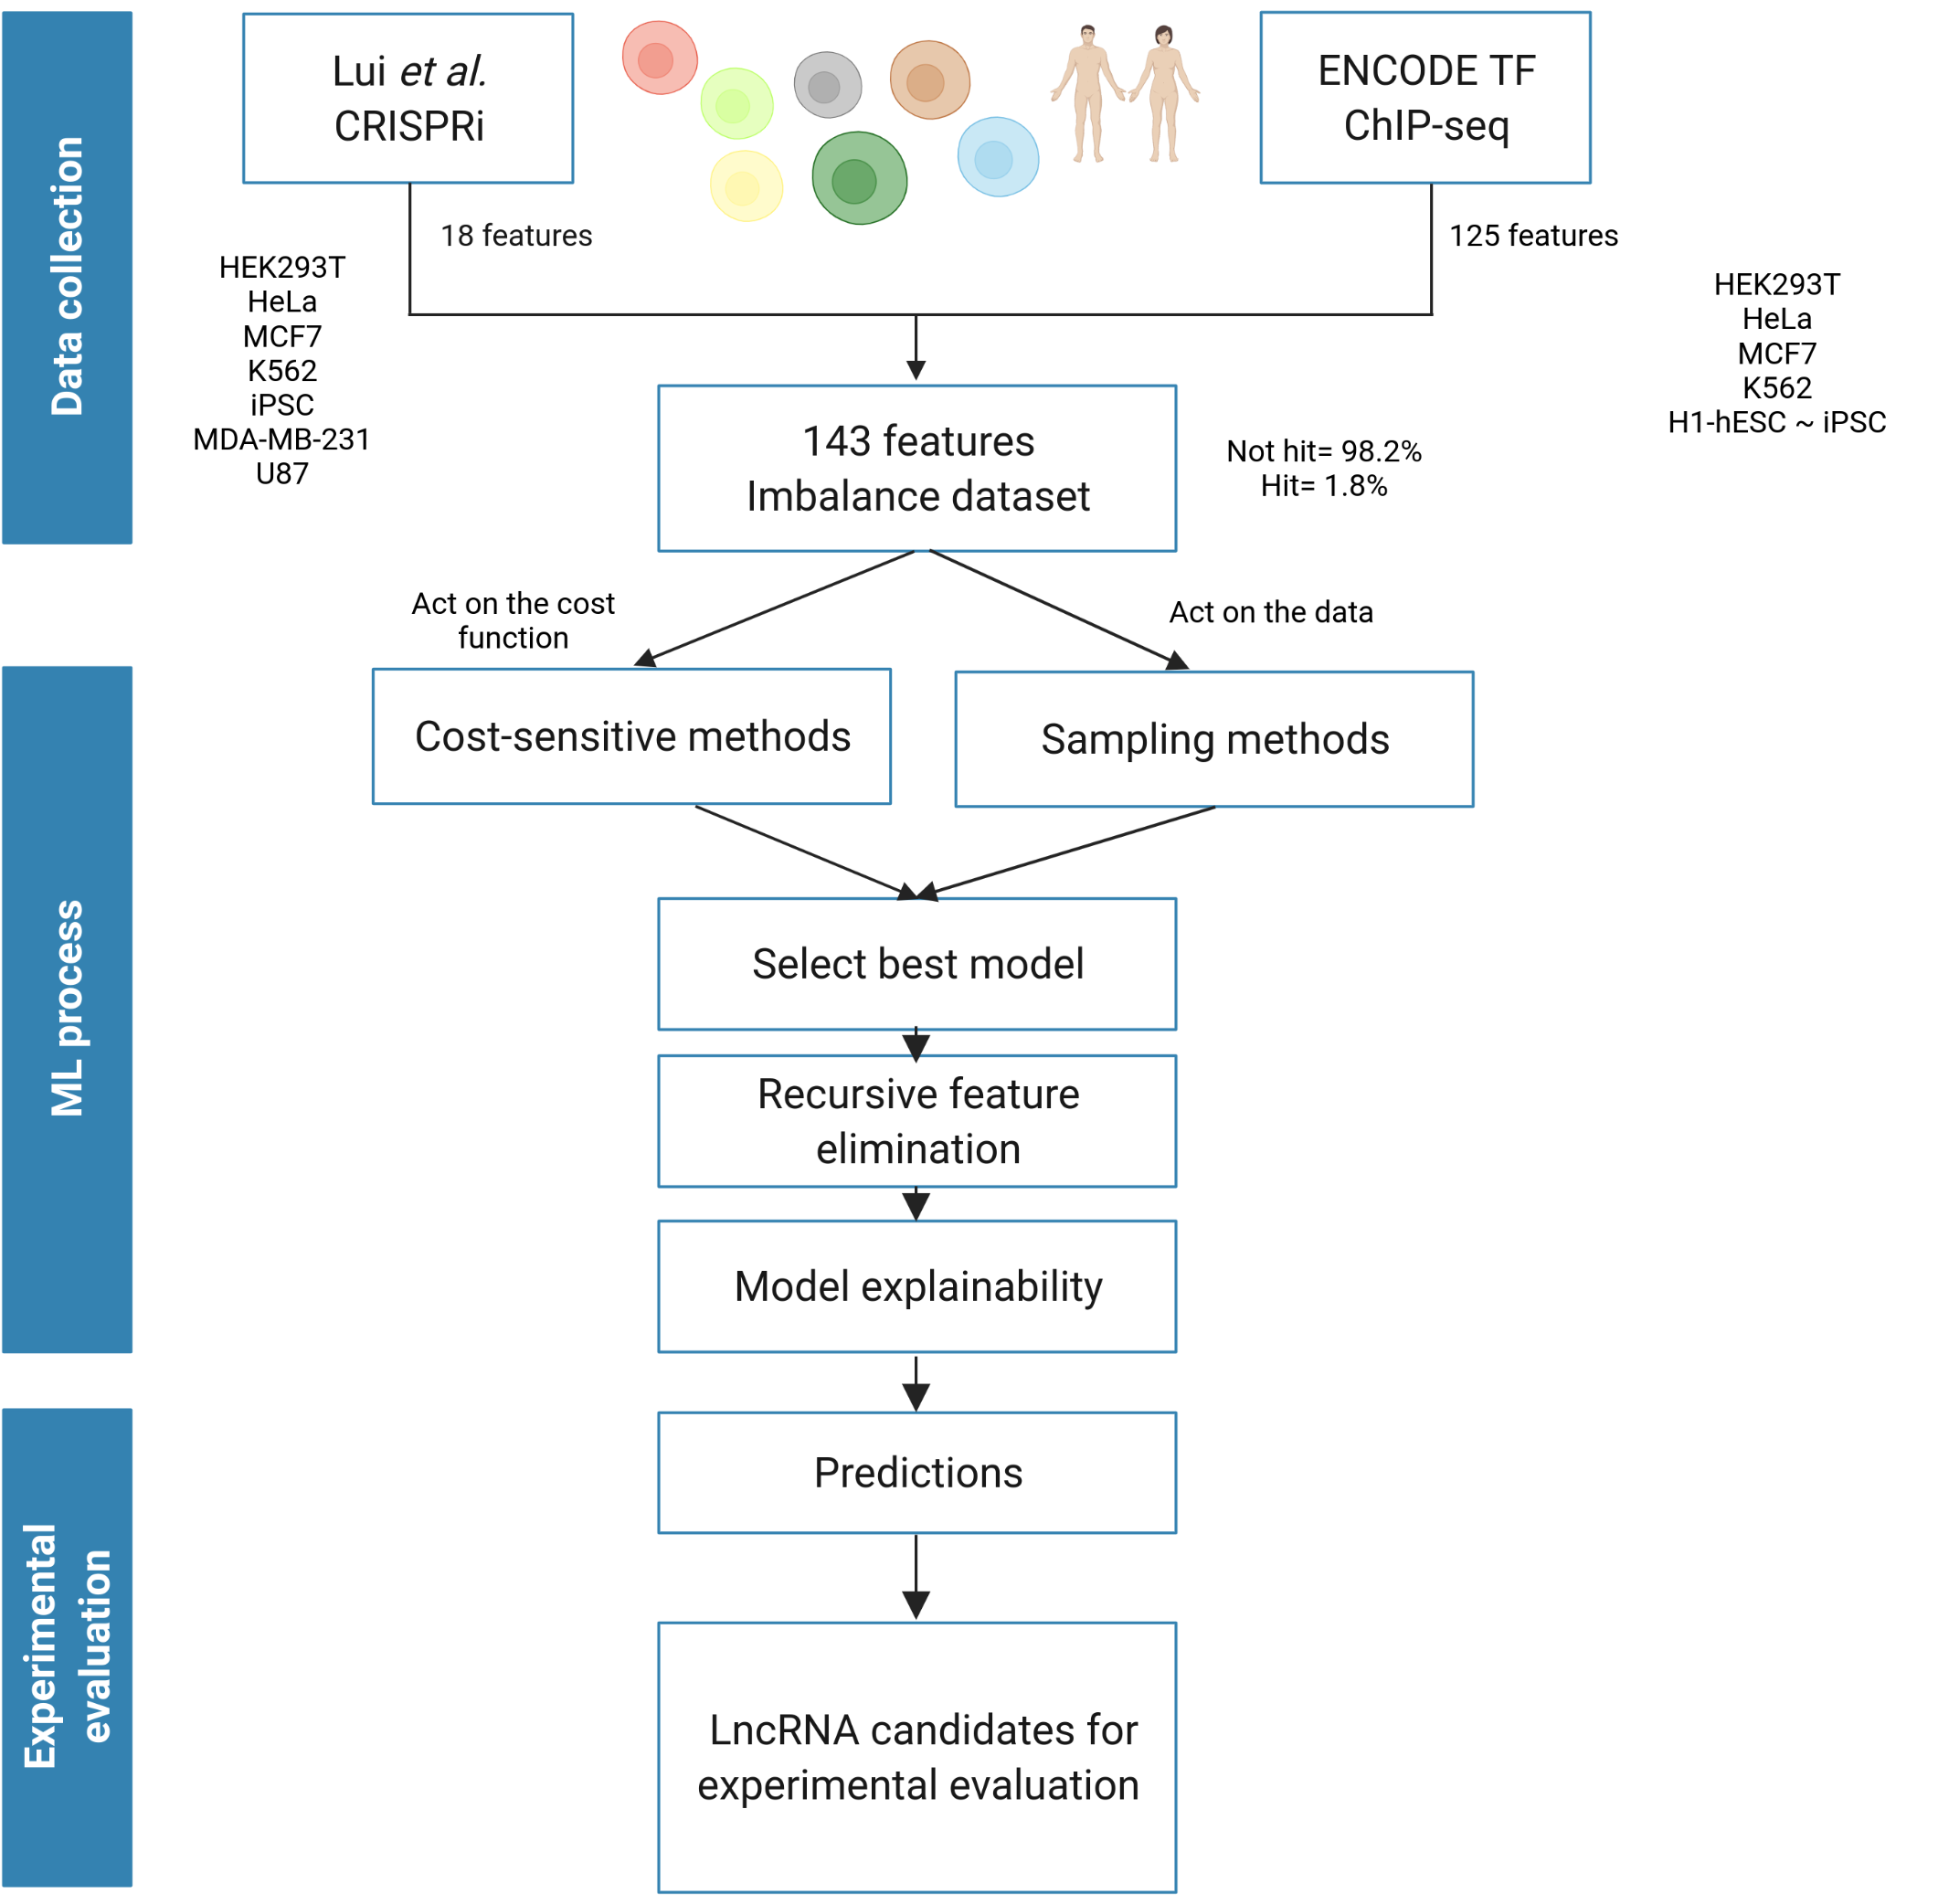
\includegraphics[width=0.9\textwidth]{img/methods/ml_project/flow_ml_lncRNA.png}
  \caption[Machine learning (ML) workflow]{\textbf{Machine learning (ML) workflow}. Processes followed to build and evaluate machine learning models, and generate candidates for experimental validation.}
  \label{fig:ml-workflow}
\end{figure}

\clearpage

\subsection{LncRNA analysis of the \textit{Drosophila} genome during regeneration}
\label{sec:noncoding-analysis-dme}

\subsubsection{Characterization of cell-damage lncRNAs}
\label{sec:chr-lncRNA-methods}

\paragraph{Mapping and quantification}
\label{sec:rna_seq_data_processiong_and_analysis}

RNA-seq regeneration data was obtained from Vizcaya-Molina \textit{et al.}\autocite{vizcaya_2018} (\autoref{tab:regeneration-dataset}). Data was processed using the \textit{grape-nf} pipeline (\url{https://github.com/guigolab/grape-nf}). RNA-seq reads were aligned to the fly genome (dm6) using \textit{STAR} \autocite{dobin_2013_star} v2.4.0j with up to 4 mismatches per paired alignment using the FlyBase genome annotation r6.29 (04 2019). Only alignments for reads mapping to ten or fewer loci were reported. Genes and transcripts were quantified in TPMs using \textit{RSEM} \autocite{li_2011_rsem} v1.2.21.  The gtf version r6.29 contains a total of 16,412 genes; 13,957 protein coding genes (PCGs) and 2,455 long noncoding RNAs (lncRNAs). In our study the lncRNAs were defined as genes > 200 bp and aligned to canonical chromosomes. See \autoref{fig:reg-ge-workflow} to have a general overview of the gene expression analysis in regeneration. 

\paragraph{Quality control of BAM files}
\label{sec:rna_seq_quality_control_of_bam_files}

Quality control of alignment sequencing data was performed using \textit{QualiMap} \autocite{garcia_2012_qualimap} v.2.2.1 and \textit{Picard} v.2.6.0 (\url{http://broadinstitute.github.io/picard/}). Using \textit{Qualimap} we obtained: number of reads, number of mapped reads, duplication rate, and GC percentage; and using \textit{Picard} we obtained: dropout, and GC dropout.

Assessment of  replicates reliability was measured with weighted correlation network analysis (WGCNA). WGCNA was implemented with the \textit{R} package \textit{WGCNA}\autocite{langfelder_wgcna} version 1.69. A cutoff of less than 2 standard deviations from a normal distribution was implemented to utilize a replicate.

\paragraph{Differential gene expression comparing: regeneration vs. control}
\label{sec:differential_expression_analysis}

Differential gene expression analyses between control and regeneration were performed separately on each time-point. Genes were filtered per time point, removing all genes with a gene expression < 1 TPM. Analyses were run using \textit{R} version 3.6.2, \textit{DESeq2}\autocite{love_2014_deseq2}, and a fold change\autocite{vizcaya_2018} approach. All genes with an absolute fold change > 1.7 in both methods were considered differentially expressed.

In addition, the PCGs \textit{rpr} and \textit{Gadd45}  were used as positive controls, and both were upregulated at the early time point. Positive controls were confirmed through qPCR (\textit{Confirmation experiments were carried out by Carlos Camilleri, from Montserrat Coromina’s lab at Universitat de Barcelona; Barcelona, Spain}).

\paragraph{Coding potential}
\label{sec:coding_potential}

The coding capability of lncRNAs was measured using \textit{CPAT}  \autocite{wang_2013_cpat} version 3.0.4. Following the developer’s indications, we took a cut-off < 0.39 to classify them as noncoding RNAs.

\paragraph{ATAC-seq analysis}
\label{sec:atac-seq-methods}

Uniquely aligned reads to canonical chromosomes from nucleosome-free data was retrieved from Vizcaya-Molina \textit{et al.}\autocite{vizcaya_2018} study. Aggregation plots around lncRNA TSS ($\pm$ 400 bp) were produced using \textit{bwtool}\autocite{pohl_bwtool} \textit{summary} version 1.0. Bed6 files were used as input to \textit{bwtool} to take into account gene strandness. LncRNA promoters were obtained using a 301 bp window centered on the main transcription start site (TSS).\autocite{batut_2017}

\paragraph{Genome-wide lncRNA classification}
\label{sec:lncRNA_classification}

LncRNA genes were classified with respect to their genome location using the classification module of the \textit{FEELnc}\autocite{wucher_2017} pipeline. \textit{FEELnc} received as input the 2,455 annotated lncRNAs from the gtf version r6.29 classifying the lncRNAs in three broad groups: \textbf{1)} intergenic (\autoref{fig:lncRNA-class}A), \textbf{2)} genic intronic (\autoref{fig:lncRNA-class}B), and \textbf{3)} genic exonic (\autoref{fig:lncRNA-class}C). The classification was mutually exclusive in the following rank: genic exonic > genic intronic > intergenic. Genic exonic and genic intronic were subcategorized as: sense or antisense, and as: overlapping, nested or containing. Intergenic were subcategorized as: same strand, divergent or convergent.

To calculate the percentage of overlapping between the genic exonic and their overlapping PCGs, we took all genic exonic pairs and their overlapping PCGs. Then using \textit{BEDTools} \autocite{quinlan_2010_bedtools} intersect v2.27, we obtained the number of base pairs that overlapped between genic-exonic exons and PCG exons and divided by the total exon length.

\begin{figure}[!htb]
  \centering
  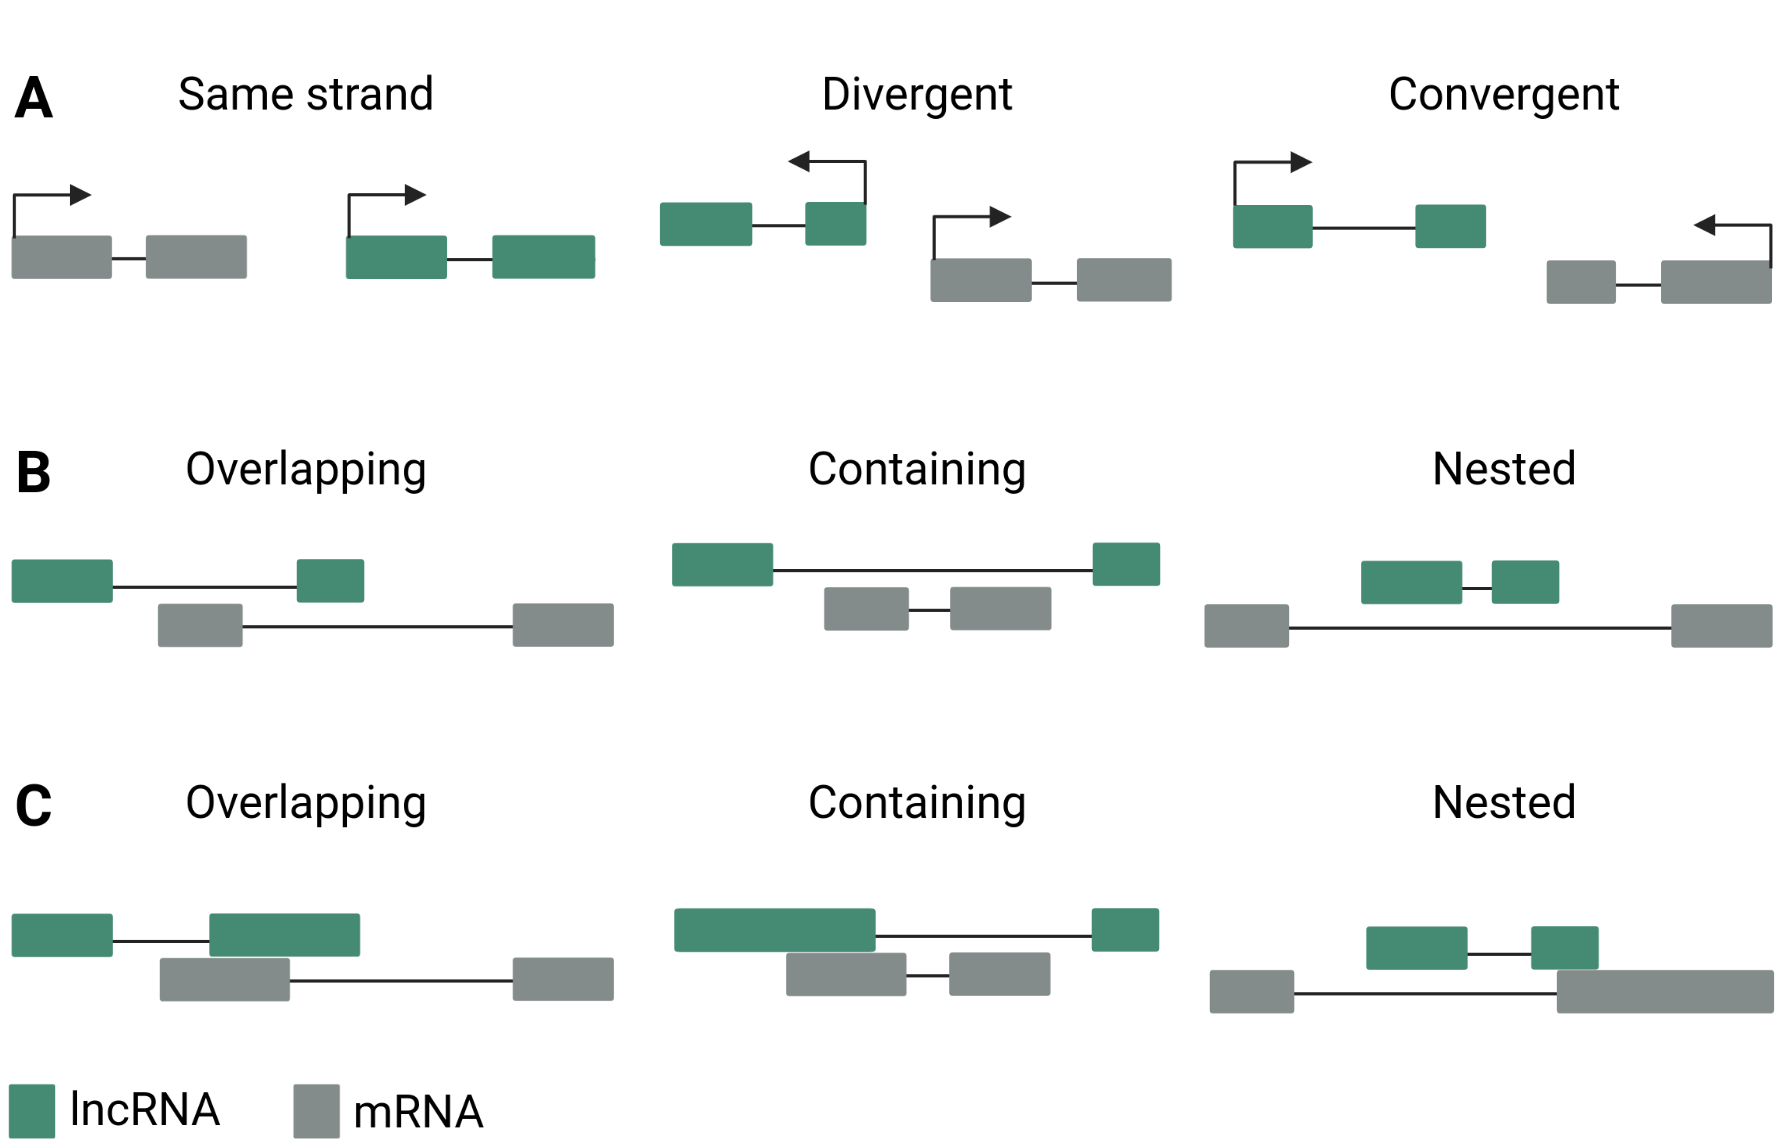
\includegraphics[width=0.7\textwidth]{img/methods/regeneration/lncRNA_class_methods.png}
  \caption[LncRNA classification]{\textbf{LncRNA classification}. \textbf{(A)} Intergenic classification. \textbf{(B)} Genic intronic and \textbf{(C)} genic exonic: overlapping, containing, and nested in sense and in antisense. Figure inspired by Wucher \textit{et al.}\autocite{wucher_2017}}
  \label{fig:lncRNA-class}
\end{figure}

\paragraph{Gene ontology enrichment}
\label{sec:gene_ontology_enrichment}

For each differentially expressed lncRNA, the expressed set of neighboring PCGs were extracted (FlyBase version r6.29). For genic (exonic and intronic) all overlapping PCGs, and for intergenic PCGs with a distance $\leq$ of 5 Kb on each side were considered (\autoref{fig:co-expression}A).

Next, the \textit{R} library \textit{clusterProfiler} \autocite{yu_2012} version 3.14.3 was used in combination with \textit{Drosophila} annotations from the \textit{R} library \textit{org.Dm.eg.db} \autocite{carlson_2013} version 3.10.0 to compute the gene ontology enrichment, using biological processes. \textit{P-values} were adjusted using \textit{FDR} multiple testing correction.

\paragraph{LncRNA:PCG co-expression analysis}
\label{sec:lncRNA_pc_co-expression}

To study the expression correlations between lncRNAs and PCGs, we used our lncRNA classification (genic exonic, genic intronic and intergenic) to automatically identify all lncRNA:PCG pairs. For long intervening noncoding RNAs (lincRNA; in this thesis work lincRNA and intergenic terms were used indistinctly), we kept all pairs that showed a locus-locus distance $\leq$ of 5 Kb up and downstream of each lincRNA, and for genic lncRNAs all their overlapping PCGs (\autoref{fig:co-expression}A).

Next, we performed a regeneration and control specific analysis, removing lncRNA:PCG pairs that were expressed < 1 TPM, in control or in regeneration, and performed two analysis: \textbf{(1)} observe the DE status of lncRNA-PCG pairs, and \textbf{(2)} classify the expression patterns of lncRNA-PCG pairs.

The DE status of lncRNA-PCG pairs consisted in classifying them as concordant or discordant. Concordant cases where defined as positive directionality (\textit{i.e.} lncRNA:upregulated and PCG:upregulated or lncRNA:downregulated and PCG:downregulated) and discordant cases were the opposite (\textit{i.e.} lncRNA:upregulated and PCG:downregulated or lncRNA:downregulated and PCG:upregulated).

For the classification of expression patterns among lncRNA-PCG pairs, increasing, decreasing, peak and valley were the implemented classes (\autoref{fig:co-expression}B). We labeled as: increasing, if the lncRNA increased its expression during the three time-points; decreasing if it decreased its expression in all time-points; peak, if the maximum expression was at the mid time-point (15h); and finally valley, if the minimum expression was at the mid time-point. 

After our classification, we retained the concordant (\textit{i.e.} lncRNA:PCG: increasing-increasing; decreasing-decreasing; peak-peak; valley-valley) and discordant cases (\textit{i.e.} lncRNA:PCG: increasing-decreasing; decreasing-increasing; peak-valley; valley-peak). In this analysis lncRNAs define the co-expression label, \textit{e.g.} concordant-valley= lncRNA is valley and neighboring PCG is valley, discordant-valley= lncRNA is valley and neighboring PCG is peak. 

\begin{figure}[!htb]
  \centering
  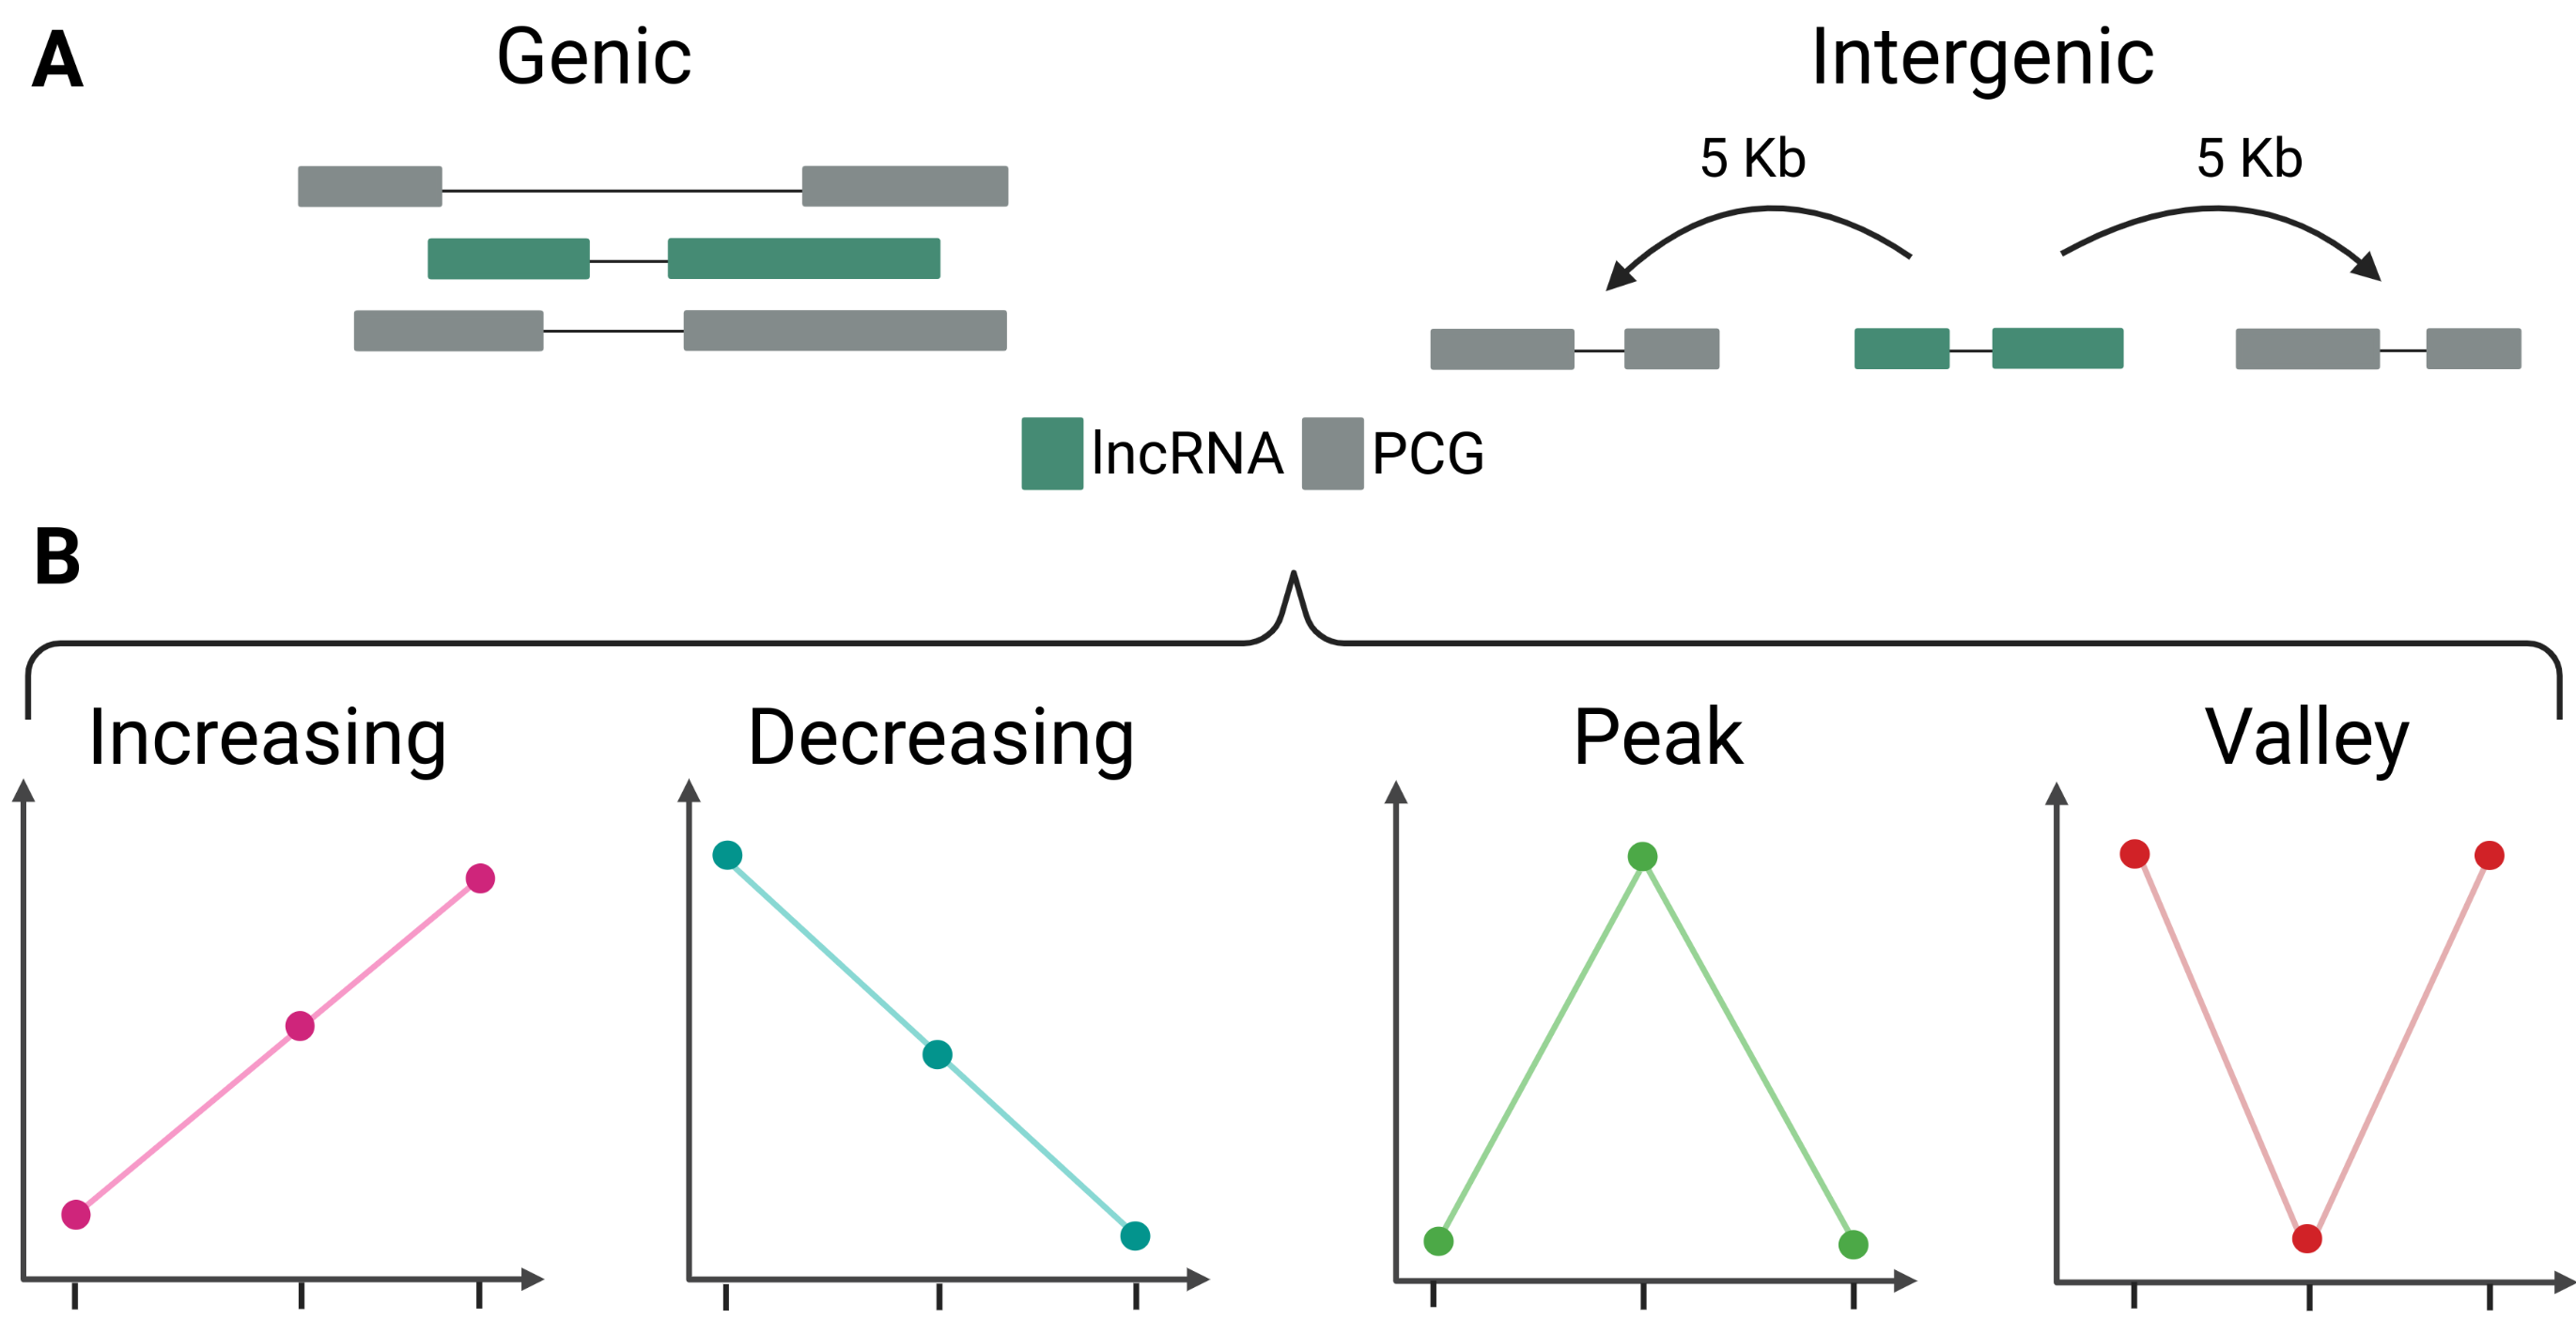
\includegraphics[width=0.8\textwidth]{img/methods/regeneration/co-expression.png}
  \caption[LncRNA:PCG co-expression analysis]{\textbf{LncRNA:PCG co-expression analysis}. \textbf{(A)} LncRNA-PCG pair selection strategy. \textbf{(B)} Co-expression classification; \textit{y-axis}= gene expression, and \textit{x-axis}: 0h, 15h, and 25h time points.}
  \label{fig:co-expression}
\end{figure}

\paragraph{LncRNA genomic features}
\label{sec:Genomic characterization}

\textit{GC} content and length of: genes, promoters, and transcripts of all lncRNA were obtained using the \textit{GC} class from \textit{Biopython}\autocite{cock_2009} version 1.78, and gtf file version r6.29. Then, \textit{Kruskal-Wallis} test was used to compare the \textit{GC} percentage and length among: lncRNA differentially expressed (DE), lncRNA expressed (in regeneration and/or control), and the rest of annotated lncRNAs. For cases with a \textit{p value} < 0.05 a pairwise Wilcoxon test was performed to obtain the \textit{p value} of each comparison. The \textit{FDR} correction method was used.

\paragraph{Sequence conservation}
\label{sec:Sequence_conservation}

LncRNA sequence conservation was obtained using the \textit{dm6} 27-way multiple alignment (23 \textit{Drosophila} sequences, house fly, \textit{Anopheles} mosquito, honey bee and red flour beetle) from the \textit{UCSC genome browser}.\autocite{tyner_2017_ucsc} Next, \textit{maf\_parse} from \textit{PHAST} \autocite{hubisz_2011_phast} v1.4 was used to do multiple alignments, and finally the maximum alignment score was taken with its respective number of aligned sequences and number of conserved species.

Two analyses were done, the first one was using the gene sequence (\textit{i.e.} exons and introns), and the second one was using the exons and then calculating the mean conservation for exons by gene. Percentage of conservation was obtained dividing the length of aligned sequences by the length of the genomic feature.

\begin{figure}[!htb]
  \centering
  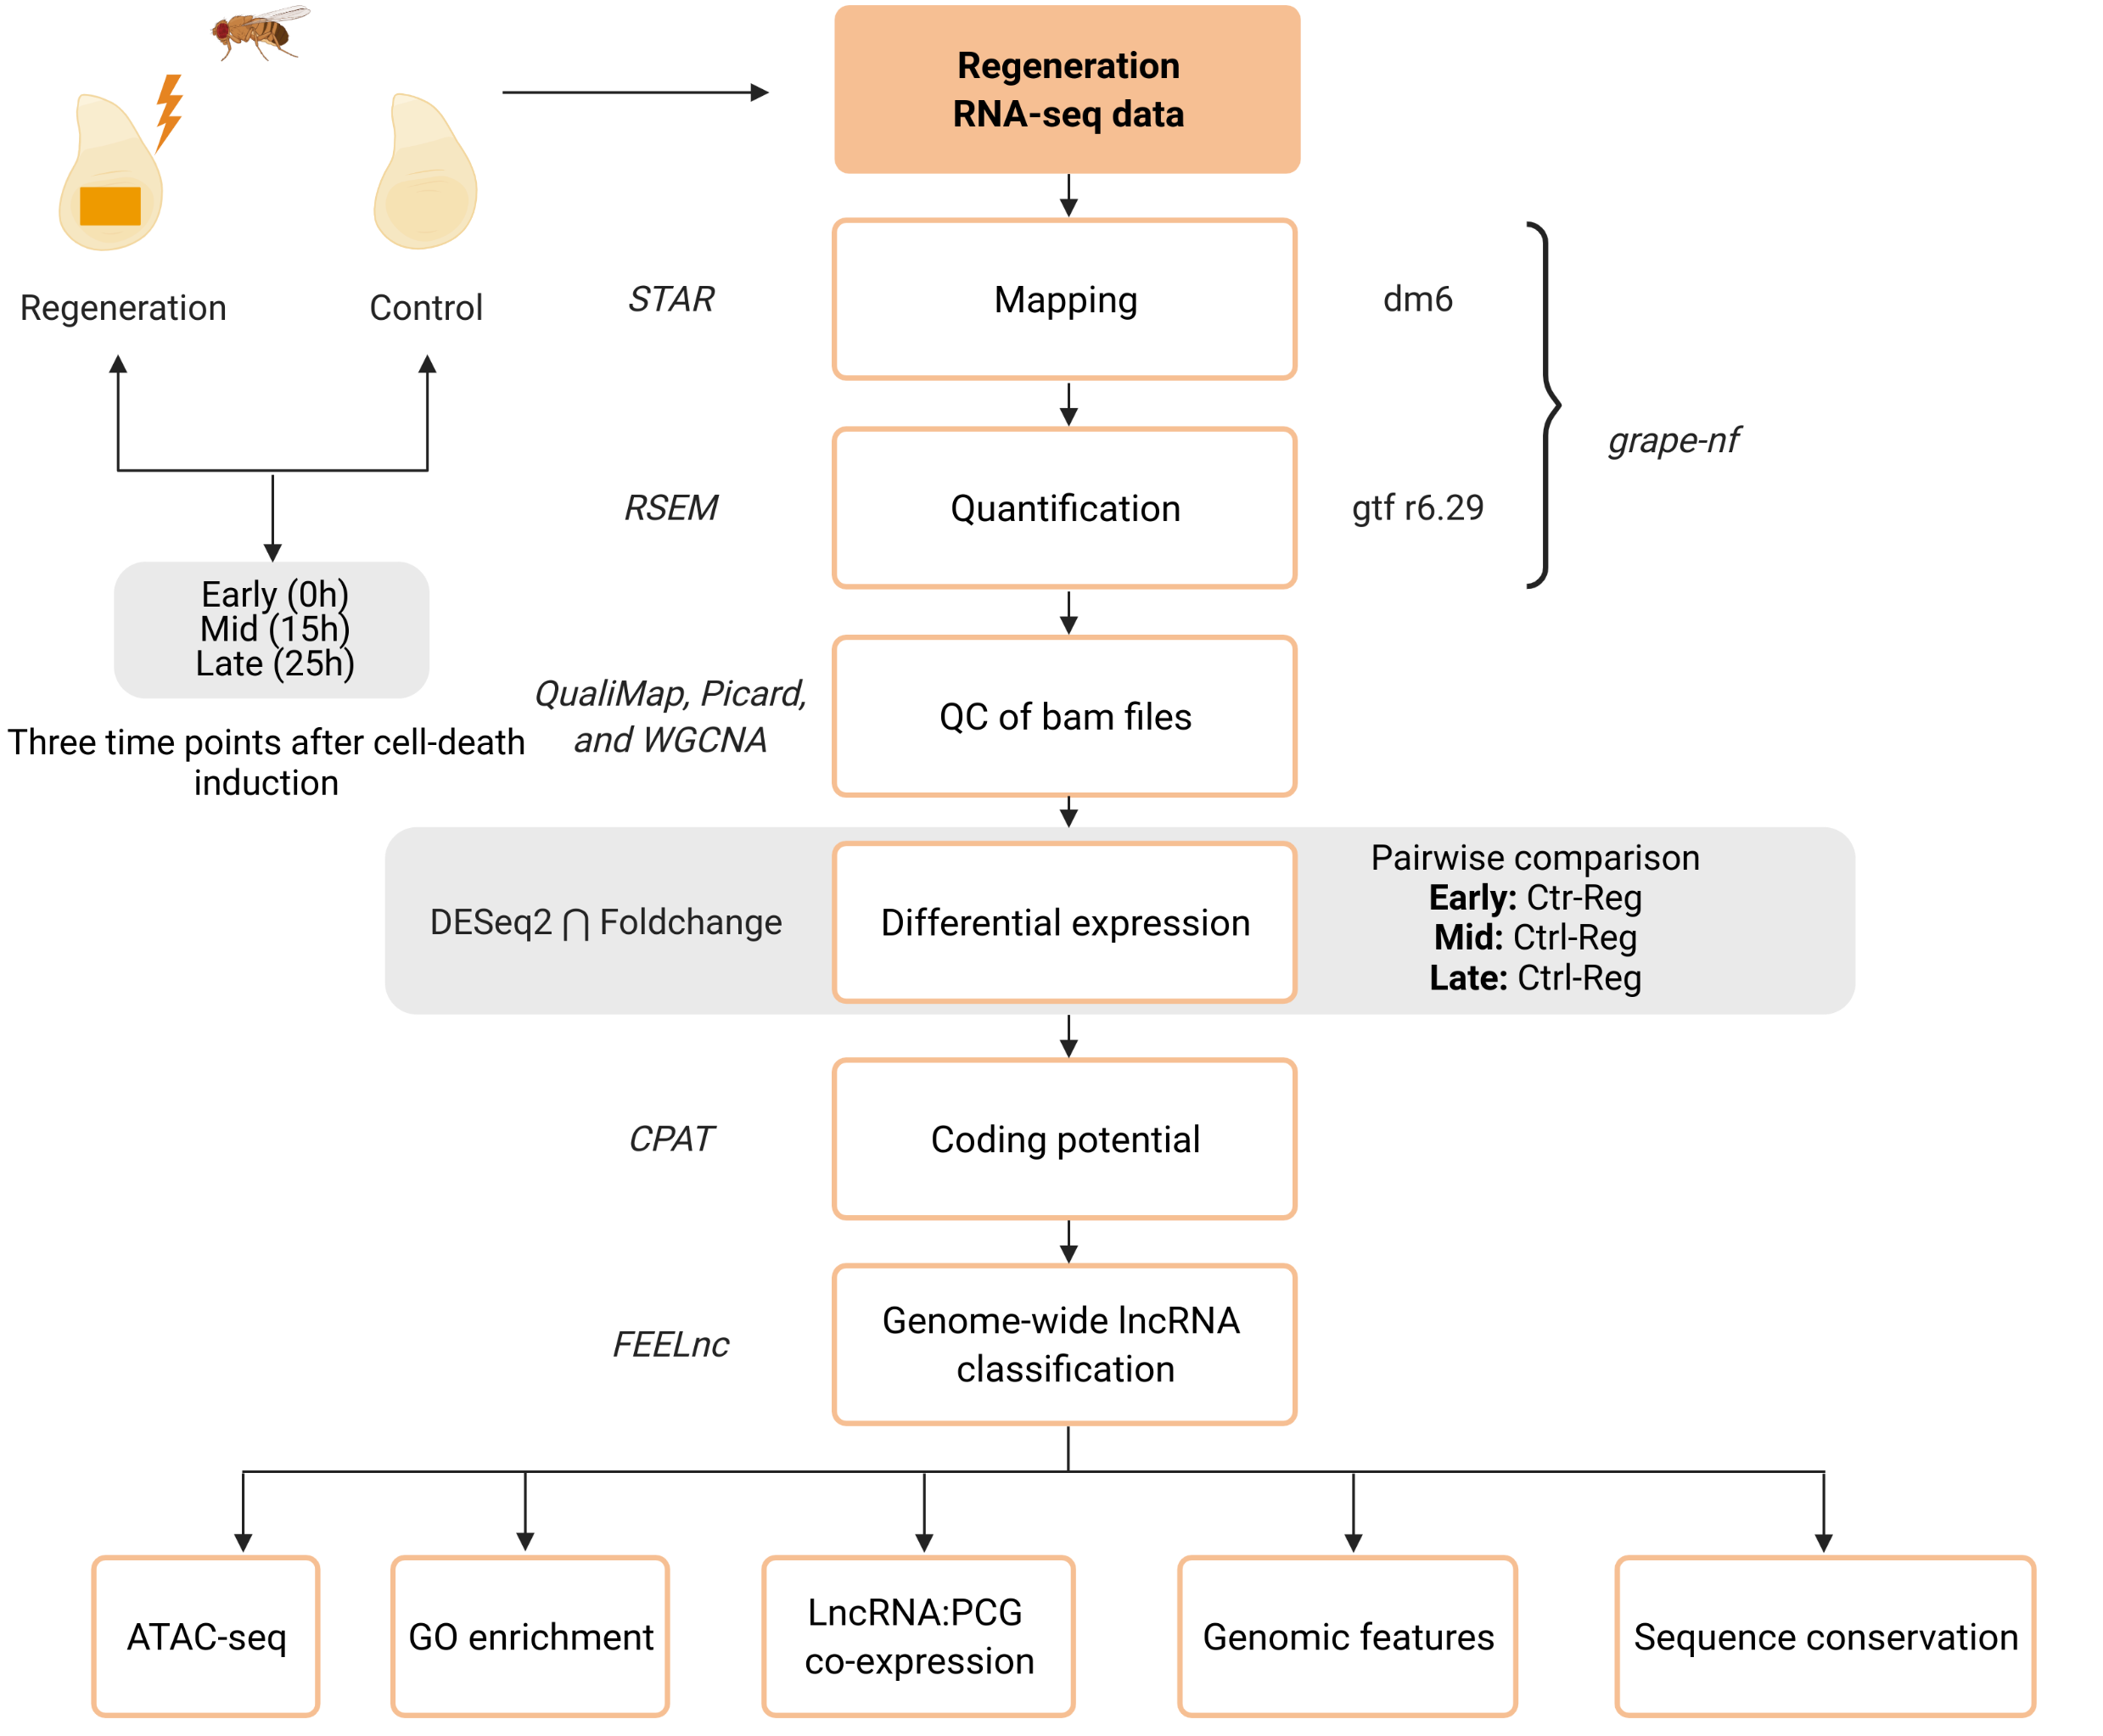
\includegraphics[width=0.95\textwidth]{img/methods/regeneration/lncRNA-pipeline-thesis.png}
  \caption[Gene expression analysis workflow]{\textbf{Gene expression analysis workflow}. LncRNA analysis of the \textit{Drosophila} genome during regeneration.}
  \label{fig:reg-ge-workflow}
\end{figure}

\clearpage

\subsubsection{LncRNA developmental and tissue signatures}
\label{sec:dme-methods-part-two}

\paragraph{Mapping, quantification, and QC}
\label{paragraph:modencode-erc-first-part}

Developmental RNA-seq data of \textit{D. melanogaster} was obtained from the modENCODE project\autocite{celniker_2009,modencode_2010} (\url{http://modencode.org/}), 21 distinct developmental stages were analyzed from embryonic to pupal stage. These stages included 12 embryonic stages divided at 2h intervals from 0h to 24h, 3 larval stages, and 6 pupal stages, with an average of 3 replicate for each stage.

\textit{D. melanogaster} leg and wing imaginal disc reads were obtained from Pérez-Lluch \textit{et al.}\autocite{perez_blister} study. Eye-antenna imaginal discs were dissected into two separated antenna and eye imaginal discs, and subsequently antenna and eye imaginal discs  were individually sequenced. (\textit{These experiments were carried out by Marina Ruiz-Romero, from Roderic Guigó’s lab at CRG; Barcelona, Spain}).  Antenna, eye, leg and wing imaginal disc data was produced for three developmental stages L3, WPP and late pupae, with 2 replicates for each imaginal disc and developmental stage. 

Developmental and imaginal disc datasets were mapped, quantified, and QC analyzed exactly as the regeneration dataset (see \nameref{sec:rna_seq_data_processiong_and_analysis} and \nameref{sec:rna_seq_quality_control_of_bam_files}). 

\paragraph{K-means clustering}
\label{paragraph:k-means-clustering}

For the cluster analysis the developmental dataset was divided in two groups: the first group (embryo-larvae group) contained the 12 embryonic stages and the three larval stages, and the second group (pupae group) contained the 6 pupal stages. 

Only lncRNAs expressed in at least one condition for the embryo-larvae group or for the pupae group were selected for the cluster analysis based on gene expression. Then, TPMs were log$_{10}$ transformed and scaled before doing the clustering.

We iteratively implemented the k-means algorithm using the \textit{R} function \textit{kmeans} and run the algorithm 10 times with random initialized centroids. Following, the clusters were filtered to remove elements with a PCA distance from the cluster centroid above cluster mean distance. Finally, we recalculated the clusters until we reached robust clusters for the embryo-larvae group and for the pupae group. 

\subsubsection{Assessing the lncRNA:\textit{CR40469} function during \textit{D. melanogaster} imaginal-disc regeneration-process}
\label{sec:cr40-methods}

\paragraph{\textit{CR40469} knockout and induction of cell-death}
\label{sec:generation_mutant_methods}

The lncRNA \textit{CR40469} was knocked-out (KO) by homozygous deletion using ends-out homologous recombination.\autocite{baena_2013} \textit{CR40469} KO (\textit{CR40469}$^{KO}$) deletion was confirmed via genomic qPCR. We used \textit{CR40469}}$^{KO}$ and \textit{CR40469} wild-type (\textit{CR40469}$^{Wt}$; Wt= wild-type) genotypes in combination with induction of cell-death at the early time point (regeneration 0h) and without induction of cell-death at the early time point (control 0h) to study the effects on gene expression. Obtaining four combinations: \textbf{(1)} \textit{CR40469}$^{KO}$ in regeneration at 0h, \textbf{(2)} \textit{CR40469}$^{KO}$ in control at 0h, \textbf{(3)} \textit{CR40469}$^{Wt}$ in regeneration at 0h, and \textbf{(4)} \textit{CR40469}$^{Wt}$ in control at 0h (see \autoref{fig:cr40469-workflow}).

Cell-death was induced using the expression of the pro-apoptotic \textit{rpr} gene according to.\autocite{santabarbara_2015,vizcaya_2018} Regeneration experiments were performed for 16h at the L3 stage in the \textit{salm} domain. In our study, control samples without \textit{rpr} expression were treated in parallel. (\textit{These experiments were carried out by Carlos Camilleri, from Montserrat Coromina’s lab at Universitat de Barcelona; Barcelona, Spain}).

\paragraph{RNA-seq library preparation, sequencing, and processing}
\label{sec:rna_seq_mutant_methods}

A total of 40 wing imaginal discs were dissected for each genotype (\textit{CR40469}$^{KO}$ and \textit{CR40469}$^{Wt}$) and cell-death condition (regeneration and control).  Three technical replicates and three independent biological replicates were performed per condition. All libraries were sequenced on Illumina HiSeq at the Ultra sequencing unit of the Centre for Genomic Regulation (CRG, Barcelona, Spain). (\textit{These experiments were carried out by Carlos Camilleri, from Montserrat Coromina’s lab at Universitat de Barcelona; Barcelona, Spain}).

Mapping, quantification, and quality control analyses were carried out using the same process described above. See \nameref{sec:rna_seq_data_processiong_and_analysis} and \nameref{sec:rna_seq_quality_control_of_bam_files} for further details.

\paragraph{Differential gene expression}
\label{sec:dge_cr40469}

We used the statistical methods implemented in the \textit{DESeq2}\autocite{love_2014_deseq2} package version 1.26.0. Only genes expressed at least 1 TPM in at least one sample were selected for this analysis. The two factors with interaction approach was implemented, using the following design matrix:  

\[ design\ matrix= model.matrix(\sim genotype + condition + genotype:condition)  \]

where genotype is \textit{CR40469}$^{KO}$ or \textit{CR40469}$^{Wt}$ and condition is regeneration or control. All genes with an absolute fold change > 1.7 and an adjusted \textit{p-value} < 0.05 were considered differentially expressed. The \textit{Benjamini-Hochberg} correction method was used. 

\begin{figure}[!htb]
  \centering
  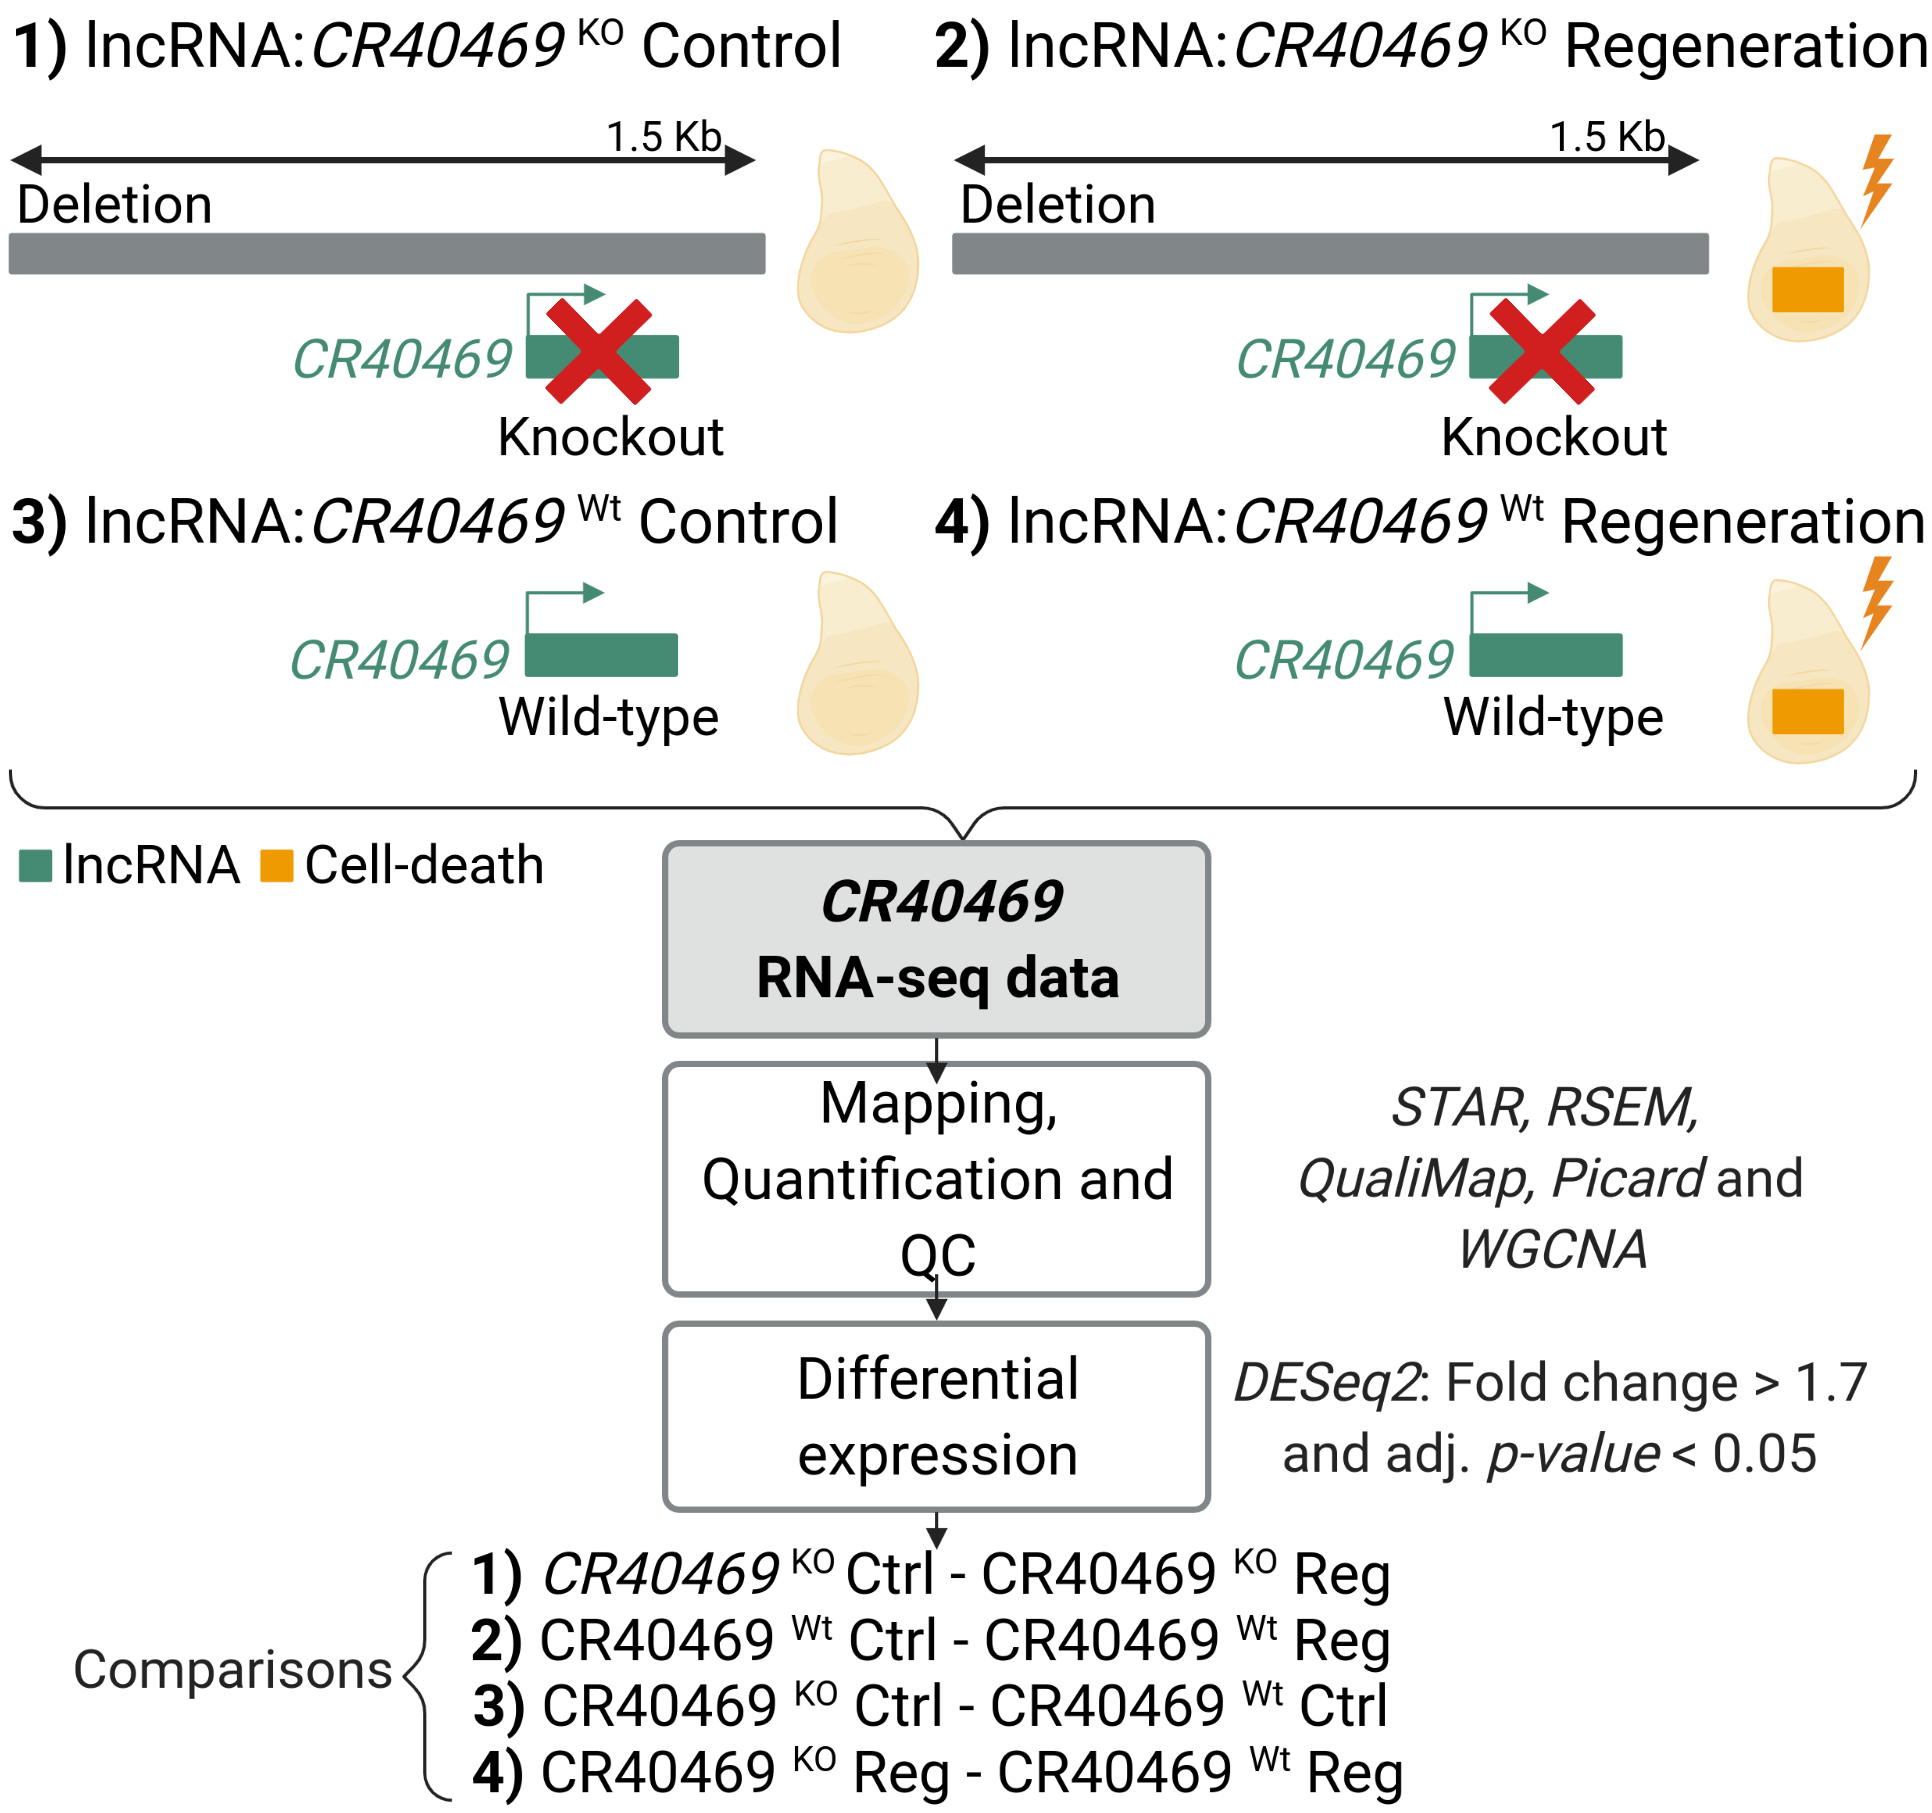
\includegraphics[width=0.7\textwidth]{img/methods/regeneration/CR40469-KO-methods.png}
  \caption[\textit{CR40469} KO analysis workflow]{\textbf{\textit{CR40469} KO analysis workflow}. Description of the four types of samples at the early time point, pipeline used to process raw reads, and the four comparisons performed for the differential expression analysis.}
  \label{fig:cr40469-workflow}
\end{figure}

